%\documentclass[french]{beamer}
\documentclass[aspectratio=169]{beamer}
\usepackage[utf8]{inputenc}
\usepackage[T1]{fontenc}
\usepackage{lmodern}
\usepackage{amsmath, amssymb}
\usepackage{babel}

\usepackage{eurosym}
%\usepackage{unicode-math}
\setbeamertemplate{footline}[frame number]

\definecolor{rouge}{HTML}{DD0000}

%Pour le TITLEPAGE

\title{Appel à projet}
\subtitle{Mardi 7 mars 2023}
\date{}
\author[N.P. - A.M. - P.T.]{Nicolas Papazoglou, Alexis Martin \& Pierre Toussaint}
\institute[ENSEA]{ENSEA}

\usetheme{ensea}  

\AtBeginSection[]
{
	\begin{frame}{Plan}
		\tableofcontents[currentsection]
	\end{frame}
}

\AtBeginSubsection[]
{
   \begin{frame}
    	\tableofcontents[currentsection,currentsubsection]
   \end{frame}
}

\begin{document}

\begin{frame}
	\titlepage
\end{frame}

\begin{frame}{Appel à projet}
\begin{minipage}{0.49\textwidth}
	\begin{itemize}
		\item Porteurs du projet : Alexis Martin, Nicolas Papazoglou, Pierre Toussaint,
		\item Demande budgétaire : 64 HETD  (répartition 50\%/25\%/25\%)
		\item Budget (DEE) : 400-500\euro / maquette
		\item Activité concernée : enseignement d'électrotechnique et d'automatique (AEI, ESE, MSC) dans un premier temps, cours de 2nde année possible dans un second temps.
	\end{itemize}
\end{minipage}
\begin{minipage}{0.49\textwidth}
	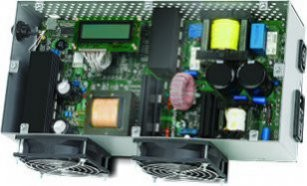
\includegraphics[scale=0.6]{figures/inverter.jpeg} 
\end{minipage}
\center \href{https://github.com/DBXYD/AAP_ENSEA_Inverter}{Lien github}
\end{frame}

%********************** OBJECTIFS ******************************
\begin{frame}{Objectif : Réalisation maquette pédagogique}
	Cibles : 
	\begin{itemize}
		\item Enseignements d'électrotechnique et automatique
	\end{itemize}
	Objectifs : 
	\begin{enumerate}
		\item Une maquette fiable et facilement réparable pour les TPs d'électrotechnique et automatique
		\item Projet open-source (disponible sur github),
		\item Compréhension globale possible par les étudiants, application de l'ensemble de leurs cours dans une maquette,
		\item Création modulaire, réutilisable dans d'autres cours/projets, 
		\item Evolution possible à d'autres enseignements (buck/boost, 4Q, brushless, moteurs synchrones, asservissement, etc...).
	\end{enumerate}
\end{frame}

\begin{frame}{Travail à effectuer}
\begin{enumerate}
	\item Cahier des charges (déjà effectué),
	\item Schéma d'architecture (déjà effectué),
	\item Choix des composants (disponibles et actuels pour une maintenibilité la plus longue possible),
	\item Prototypage et tests unitaires électriques,
	\item Réalisation software et tests complets,
	\item Réalisation mécanique (boitier),
	\item Intégration complète,
	\item Documentation (github),
\end{enumerate}
\end{frame}

\begin{frame}{Travail déjà effectué : Cahier des charges}
\begin{itemize}
	\item Onduleur triphasé 60V / 15A
	\item Protections surtensions et surintensités
	\item Commande de mise sous tension
	\item Commande UART
	\item Utilisable en commande ``brushless'' :  entrées position ``hall'' 
	\item Utilisable en commande vectorielle + MCC : entrée position ``encoder''
	\item Protection alimentation non réversible : module ``freinage''
	\item Vérification des temps morts
	\item Mesure de courants (hall) dans les 3 phases + entrée
	\item Mesure de tension dans les 3 phases + entrée
	\item Alimentation externe secteur
	\item Affichage erreurs (LEDs) + intensité PWM (LEDs)
	\item Sorties mesures de courants + PWMs
	\item Boitier
	\item Tenue thermique
	\item Isolation galvanique
\end{itemize}
\end{frame}

\begin{frame}{Travail déjà effectué : Schéma d'architecture}
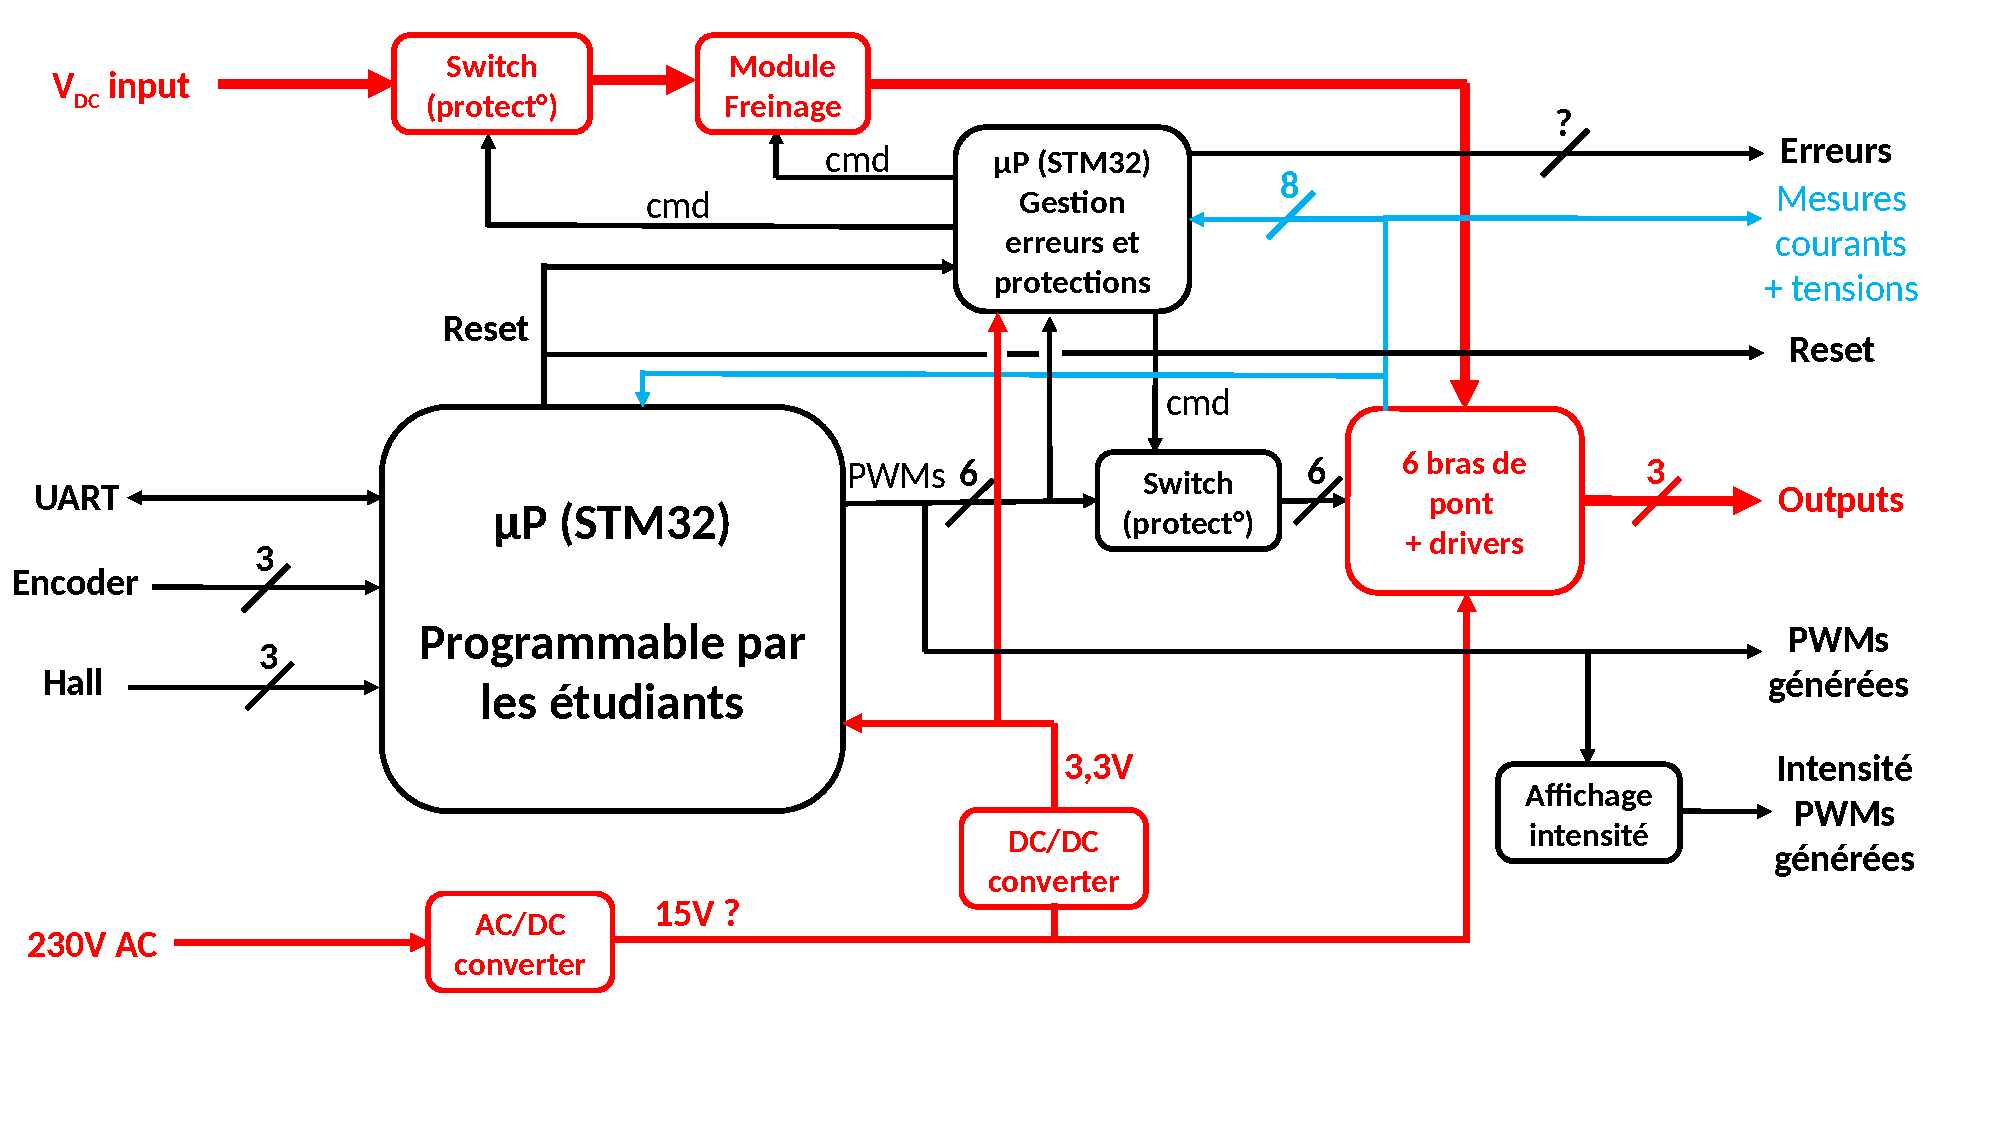
\includegraphics[width=\linewidth]{figures/Schema_architecture.pdf} 
\end{frame}

\begin{frame}{Dead-line et rémunération}
\begin{itemize}
	\item Prototype fonctionnel pour la rentrée de septembre 2023,
	\item Rémunération demandée : 64 HETD.
\end{itemize}

\end{frame}

\end{document}